\section{\uppercase{Related Work}}
\label{sec:related-work}

Research on multi–temporal BCD has progressed rapidly with the rise of deep learning and the availability of large–scale satellite datasets. A broad spectrum of architectures has been proposed, ranging from early convolutional siamese designs \cite{Daudt2018SiamICIP,Yang2021DeepSiamese,Guo2021DBFUpdate,Cao2023FFCTL,Xiao2024CSCLNet} to more elaborate encoder–decoder formulations tailored for urban structures \cite{Zhao2023DualEncoderDecoder,Tan2024SCM}. More recent efforts focus on Transformer-based bi–temporal reasoning \cite{Fang2021SNUNetCD,Chen2022BIT,Bandara2022ChangeFormer,Zheng2022HFANet,Teng2023SwinCD}, which model long-range spatial–temporal interactions more effectively than CNN-based counterparts. Complementarily, a rich line of work on efficient attention \cite{Katharopoulos2020Linear,Choromanski2021Performer,Wang2020Linformer,Xiong2021Nystromformer,Liu2021Swin,Wei2023Sparsifiner} seeks to mitigate the quadratic complexity of MHSA. These trends motivate the development of RALA–ChangeFormer.


\noindent \textbf{Transformer-Based Building Change Detection}. Early deep learning methods for BCD relied on convolutional Siamese networks with feature differencing and multi–scale fusion modules, including STANet and SNUNet–CD \cite{Fang2021SNUNetCD,Zheng2020LEVIR}. Transformer–based architectures subsequently improved performance by modeling long–range spatial–temporal dependencies. BIT introduced cross–temporal interaction via bidirectional attention \cite{Chen2022BIT}, ChangeFormer \cite{Bandara2022ChangeFormer} combined hierarchical CNN encoders with lightweight Transformer blocks, and HFA–Net refined multi–scale feature aggregation with high–frequency attention \cite{Zheng2022HFANet}. More recent efforts such as Swin–based BCD models \cite{Teng2023SwinCD} further highlight the benefit of global receptive fields. Despite these advances, all such models rely on full Multi–Head Self–Attention (MHSA) \cite{Vaswani2017Attention}, whose quadratic complexity becomes prohibitive for VHR imagery.


\begin{figure*}[t]
    \centering
    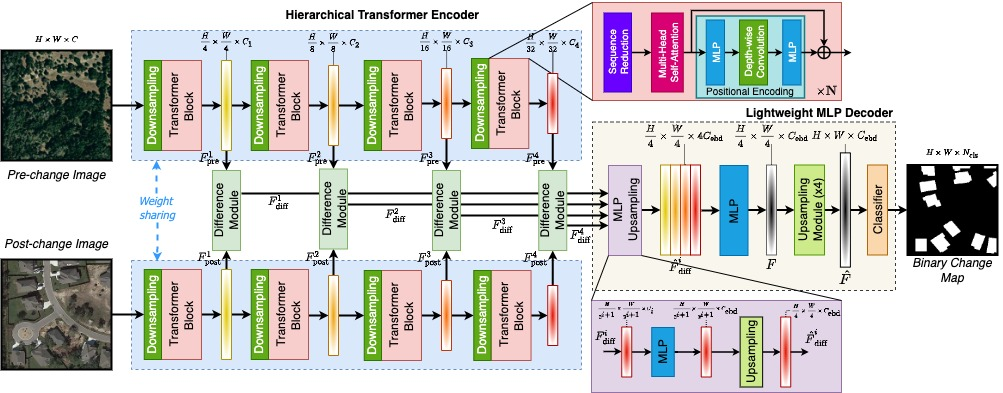
\includegraphics[width=\textwidth]{images/IGARS_ChangeFormer.jpeg}
    \caption{Overview of the baseline ChangeFormer architecture. Recovery from ChangeFormer original paper \cite{Bandara2022ChangeFormer}}
    \label{fig:changeformer_architecture}
\end{figure*}


\noindent \textbf{Efficient and Linear Attention Mechanisms}.  
To mitigate the quadratic cost of MHSA \cite{Vaswani2017Attention}, several efficient attention mechanisms have been proposed. Kernelized linear attention methods, including the Performer \cite{Choromanski2021Performer} and Linear Transformers \cite{Katharopoulos2020Linear}, replace softmax attention with feature maps to achieve $\mathcal{O}(N)$ complexity. Low–rank approximations such as Linformer \cite{Wang2020Linformer} and Nyströmformer \cite{Xiong2021Nystromformer} reduce computation by projecting the attention matrix into lower–dimensional spaces. Windowed or sparse variants (e.g., Swin Transformer \cite{Liu2021Swin} and Sparsifiner \cite{Wei2023Sparsifiner}) restrict token interactions to learned or structured neighborhoods. Although effective in some vision tasks, these approaches often suffer from reduced feature diversity due to inherent low–rank behavior, which limits performance in dense prediction tasks such as semantic segmentation. Rank–Augmented Linear Attention (RALA) \cite{Fan2025RALA} directly addresses this issue by increasing the rank of the key–value representation through token–wise weighting and output modulation.

\noindent \textbf{Gap in the Literature}.  
Despite progress in both BCD architectures and efficient attention mechanisms, rank–augmented linear attention has not been explored in multi–temporal remote sensing. Existing BCD Transformers still depend on full MHSA \cite{Vaswani2017Attention}, which constrains scalability to high resolutions and limits feasible batch sizes. Likewise, prior efficient attention techniques have not been systematically evaluated under the spatial–temporal constraints of bi–temporal BCD. This motivates the integration of RALA into a BCD architecture to improve efficiency while maintaining segmentation accuracy.